\PassOptionsToPackage{unicode=true}{hyperref} % options for packages loaded elsewhere
\PassOptionsToPackage{hyphens}{url}
\PassOptionsToPackage{dvipsnames,svgnames*,x11names*}{xcolor}
%
\documentclass[]{article}
\usepackage{lmodern}
\usepackage{amssymb,amsmath}
\usepackage{ifxetex,ifluatex}
\usepackage{fixltx2e} % provides \textsubscript
\ifnum 0\ifxetex 1\fi\ifluatex 1\fi=0 % if pdftex
  \usepackage[T1]{fontenc}
  \usepackage[utf8]{inputenc}
  \usepackage{textcomp} % provides euro and other symbols
\else % if luatex or xelatex
  \usepackage{unicode-math}
  \defaultfontfeatures{Ligatures=TeX,Scale=MatchLowercase}
\fi
% use upquote if available, for straight quotes in verbatim environments
\IfFileExists{upquote.sty}{\usepackage{upquote}}{}
% use microtype if available
\IfFileExists{microtype.sty}{%
\usepackage[]{microtype}
\UseMicrotypeSet[protrusion]{basicmath} % disable protrusion for tt fonts
}{}
\IfFileExists{parskip.sty}{%
\usepackage{parskip}
}{% else
\setlength{\parindent}{0pt}
\setlength{\parskip}{6pt plus 2pt minus 1pt}
}
\usepackage{xcolor}
\usepackage{hyperref}
\hypersetup{
            pdftitle={LTE Cat-NB (Narrowband) Performance Evaluation},
            pdfauthor={Daniel Robinson},
            colorlinks=true,
            linkcolor=blue,
            citecolor=Blue,
            urlcolor=Blue,
            breaklinks=true}
\urlstyle{same}  % don't use monospace font for urls
\usepackage[left=3cm,right=3cm,top=2cm,bottom=2cm]{geometry}
\usepackage{longtable,booktabs}
% Fix footnotes in tables (requires footnote package)
\IfFileExists{footnote.sty}{\usepackage{footnote}\makesavenoteenv{longtable}}{}
\usepackage{graphicx,grffile}
\makeatletter
\def\maxwidth{\ifdim\Gin@nat@width>\linewidth\linewidth\else\Gin@nat@width\fi}
\def\maxheight{\ifdim\Gin@nat@height>\textheight\textheight\else\Gin@nat@height\fi}
\makeatother
% Scale images if necessary, so that they will not overflow the page
% margins by default, and it is still possible to overwrite the defaults
% using explicit options in \includegraphics[width, height, ...]{}
\setkeys{Gin}{width=\maxwidth,height=\maxheight,keepaspectratio}
\setlength{\emergencystretch}{3em}  % prevent overfull lines
\providecommand{\tightlist}{%
  \setlength{\itemsep}{0pt}\setlength{\parskip}{0pt}}
\setcounter{secnumdepth}{5}
% Redefines (sub)paragraphs to behave more like sections
\ifx\paragraph\undefined\else
\let\oldparagraph\paragraph
\renewcommand{\paragraph}[1]{\oldparagraph{#1}\mbox{}}
\fi
\ifx\subparagraph\undefined\else
\let\oldsubparagraph\subparagraph
\renewcommand{\subparagraph}[1]{\oldsubparagraph{#1}\mbox{}}
\fi

% set default figure placement to htbp
\makeatletter
\def\fps@figure{htbp}
\makeatother

\usepackage{float}
\usepackage{graphicx}
\usepackage{subfig}
\usepackage{chngcntr}

\counterwithin{figure}{section}

\let\origfigure\figure
\let\endorigfigure\endfigure
\renewenvironment{figure}[1][2] {
    \expandafter\origfigure\expandafter[H]
} {
    \endorigfigure
}

%% pandoc-tablenos: required package
\usepackage{caption}

%% pandoc-tablenos: environment to disable table caption prefixes
\makeatletter
\newcounter{tableno}
\newenvironment{tablenos:no-prefix-table-caption}{
    \caption@ifcompatibility{}{
    \let\oldthetable\thetable
    \let\oldtheHtable\theHtable
    \renewcommand{\thetable}{tableno:\thetableno}
    \renewcommand{\theHtable}{tableno:\thetableno}
    \stepcounter{tableno}
    \captionsetup{labelformat=empty}
    }
}{
    \caption@ifcompatibility{}{
    \captionsetup{labelformat=default}
    \let\thetable\oldthetable
    \let\theHtable\oldtheHtable
    \addtocounter{table}{-1}
    }
}
\makeatother

\title{LTE Cat-NB (Narrowband) Performance Evaluation}
\author{Daniel Robinson}
\date{Stellenbosch University, Sept 2019}

\begin{document}
\maketitle
\begin{abstract}
2G/GPRS is a sun-setting technology leaving behind a void for LPWANs
such as LoRaWAN and SigFox to fill. The viability of NB-IoT being such a
technology for South Africa is investigated. Multiple endpoint
manufacturers and base station vendors are tested to compare
capabilities with respect to power efficiency, latency, signal strength
and other metrics. The results proved promising.
\end{abstract}

{
\hypersetup{linkcolor=}
\setcounter{tocdepth}{3}
\tableofcontents
}
\listoftables
\listoffigures
\begin{figure}
\centering

\includegraphics{../images/whitespace.png}
\caption{}
\end{figure}

\newpage

\hypertarget{declaration}{%
\section*{Declaration}\label{declaration}}
\addcontentsline{toc}{section}{Declaration}

By submitting this report electronically, I declare that the entirety of
the work contained therein is my own, original work, that I am the sole
author thereof (save to the extent explicitly otherwise stated), that
reproduction and publication thereof by Stellenbosch University will not
infringe any third party rights and that I have not previously in its
entirety or in part submitted it for obtaining any qualification.

\vspace{1cm}

Date:
\ldots{}\ldots{}\ldots{}\ldots{}\ldots{}\ldots{}\ldots{}\ldots{}\ldots{}\ldots{}\ldots{}\ldots{}\ldots{}\ldots{}\ldots{}\ldots{}\ldots{}\ldots{}.

\vspace{15cm}

Copyright © 2020 Stellenbosch University

All rights reserved.

\newpage

\hypertarget{abstract}{%
\section*{Abstract}\label{abstract}}
\addcontentsline{toc}{section}{Abstract}

A number of tests have been developed, performed and analyzed for
multiple UEs (Ublox and Quectel) and MNOs (MTN and Vodacom) via ZTE and
Nokia vendors. Power saving, latency, RF, packet and network metrics are
evaluated using UDP, Echo, COPS (network registration), eDRX and PTAU
tests.

\hypertarget{uittreksel}{%
\section*{Uittreksel}\label{uittreksel}}
\addcontentsline{toc}{section}{Uittreksel}

\hypertarget{acknowledgements}{%
\section*{Acknowledgements}\label{acknowledgements}}
\addcontentsline{toc}{section}{Acknowledgements}

\begin{itemize}
\tightlist
\item
  \textbf{Prof Thinus Booysen} - for his unrelenting care, innovative
  passion, inspiring belief in people and charming charisma.
\item
  \textbf{Family} - for their love and dedication.
\item
  \textbf{Friends} - for their wisdoms, experiencing the journey
  together and sharing moments in highs and lows.
\item
  \textbf{MTN Mobile Intelligence Lab} - for providing funding,
  expertise and laboratory working environment.
\item
  \textbf{Ryan van den Bergh} - for driving innovative ideas at MTN.
\item
  \textbf{Michael Beetge} - for his expertise in the MTN Phase 3: Test
  Plant and extensive knowledge of LTE
\item
  \textbf{Collin Mamdoo} - for his knowledge on IoT and helpful
  assistance at Vodacom
\item
  \textbf{Helene Lambrechts} - for her aid in coherence and cohesion.
\item
  \textbf{RF Design} - for providing samples and development kits.
\end{itemize}

\hypertarget{acronyms}{%
\section*{Acronyms}\label{acronyms}}
\addcontentsline{toc}{section}{Acronyms}

\begin{tablenos:no-prefix-table-caption}

\begin{longtable}[]{@{}ll@{}}
\toprule
\endhead
\textbf{3GPP} & Third Generation Partnership Project\tabularnewline
\textbf{AMQP} & Advanced Message Queue Protocol\tabularnewline
\textbf{AMOS} & Advanced Managed Object Script\tabularnewline
\textbf{AT} & Attention\tabularnewline
\textbf{BPSK} & Binary Phase-Shift Keying\tabularnewline
\textbf{BTS} & Base Transceiver Station\tabularnewline
\textbf{CDP} & Connected Device Platform\tabularnewline
\textbf{COPS} & Cellular Operator Selection\tabularnewline
\textbf{CoAP} & Constrained Application Protocol\tabularnewline
\textbf{D2D} & Device to Device\tabularnewline
\textbf{DCE} & Data Communications Equipment\tabularnewline
\textbf{DL} & Downlink\tabularnewline
\textbf{DTE} & Data Terminal Equipment\tabularnewline
\textbf{E-UTRAN} & Evolved-UMTS Terrestrial Radio Access
Network)\tabularnewline
\textbf{EARFCN} & E-UTRA Absolute Radio Frequency Channel
Number\tabularnewline
\textbf{EARFCN} & Extended Absolute Radio-Frequency Channel
Number\tabularnewline
\textbf{ECL} & Enhanced Coverage Level\tabularnewline
\textbf{eDRX} & Extended Discontinuous Receive\tabularnewline
\textbf{eNB - eNodeB} & E-UTRAN Node B\tabularnewline
\textbf{GPRS} & General Packet Radio Service\tabularnewline
\textbf{ICT} & Information and Communications Technology\tabularnewline
\textbf{IMEI} & International Mobile Equipment Identity\tabularnewline
\textbf{IMSI} & International Mobile Station Identity\tabularnewline
\textbf{IP} & Internet Protocol\tabularnewline
\textbf{LBT} & Listen Before Talk\tabularnewline
\textbf{LPWAN} & Low-Power Wide-Area-Network\tabularnewline
\textbf{LTE Cat-NB1/2} & Long Term Evolution Narrow-Band Category
1/2\tabularnewline
\textbf{MCL} & Maximum Coupling Link\tabularnewline
\textbf{MCS} & Message Coding Scheme\tabularnewline
\textbf{MNO} & Mobile Network Operator\tabularnewline
\textbf{MO} & Mobile Originated\tabularnewline
\textbf{MO} & Managed Object\tabularnewline
\textbf{MQTT} & Message Queuing Telemetry Transport\tabularnewline
\textbf{MT} & Mobile Terminated\tabularnewline
\textbf{MTC} & Machine Type Communications\tabularnewline
\textbf{MTN} & Mobile Telephone Network\tabularnewline
\textbf{NW} & Network\tabularnewline
\textbf{OTDOA} & Observed Time Difference Of Arrival\tabularnewline
\textbf{PCI} & Physical Channel ID\tabularnewline
\textbf{PDR} & Packet Delivery Ratio\tabularnewline
\textbf{PS} & Packet Switched\tabularnewline
\textbf{PTAU} & Periodic Tracking Area Update\tabularnewline
\textbf{PTAU} & Periodic Tracking Area Update\tabularnewline
\textbf{QXDM} & QUALCOMM eXtensible Diagnostic Monitor\tabularnewline
\textbf{RRC} & Radio Resource Control\tabularnewline
\textbf{SIM} & Subscriber Identity Module\tabularnewline
\textbf{SMS} & Short Message Service\tabularnewline
\textbf{SNR} & Signal to Noise Ratio\tabularnewline
\textbf{TCP} & Transmission Control Protocol\tabularnewline
\textbf{TE} & Terminal Equipment\tabularnewline
\textbf{UDP} & User Datagram Protocol\tabularnewline
\textbf{UE} & User Equipment\tabularnewline
\textbf{UL} & Uplink\tabularnewline
\textbf{UMTS} & Universal Mobile Telecommunications
System\tabularnewline
\textbf{URC} & Unsolicited Result Code\tabularnewline
\textbf{USSD} & Unstructured Supplementary Service Data\tabularnewline
\textbf{UUID} & Unique User Identification\tabularnewline
\textbf{WAP} & Wireless Application Protocol\tabularnewline
\bottomrule
\end{longtable}

\end{tablenos:no-prefix-table-caption}

\hypertarget{siunits}{%
\subsection*{SI Units}\label{siunits}}
\addcontentsline{toc}{subsection}{SI Units}

\begin{itemize}
\tightlist
\item
  \textbf{kB, MB} - kilobyte, megabyte
\item
  \textbf{kbps} - kilobits per second
\item
  \textbf{mJ or J} - millijoules or joules
\item
  \textbf{s, ms, us} - second, millisecond, microsecond
\item
  \textbf{mWh} - average power in milliwatt-hours
\end{itemize}

\newpage

\hypertarget{intro}{%
\section{Introduction}\label{intro}}

Narrowing the spectrum bandwidth for LTE results in a low
data-throughput, low energy technology which matches the requirements
for wireless IoT, hence NB-IoT.

This chapter introduces the reader to various concepts relating to
NB-IoT and the performance characteristics thereof. It begins with the
question ``Why NB-IoT?'' before developing the research question,
objectives, scope, terminology, background and other various related
concepts to fully orient the reader with regards to NB-IoT.

\hypertarget{why}{%
\subsection{Why NB-IoT?}\label{why}}

NB-IoT is an LTE technology developed by the 3GPP as a response to the
growing need for an LPWAN to fill the role 2G/GPRS leaves behind as
countries around the world schedule its departure. The technology shows
performance benefits over alternative LPWANS in terms of up and downlink
throughput, range and longevity, yet current research shows that
variation in energy consumption leaves battery longevity in question.
Nevertheless, according to 3GPP specifications and manufacturer claims,
highlights include:

\begin{itemize}
\tightlist
\item
  \textasciitilde{} 10 year battery-lifetime.
\item
  Under 10 second transmission acknowledgement for latency-tolerant
  applications
\item
  + 20 dB improvement over 2G/GPRS via enhanced coverage levels (ECL).
\end{itemize}

It would be useful to further investigate variation in energy
consumption in the technology.

\hypertarget{probstat}{%
\subsection{Problem Statement}\label{probstat}}

Knowing that NB-IoT (LTE Cat-NB) is a competitive alternative to
LoRaWAN, SigFox and other LPWANs, it does not have strong uptake in
South Africa yet. It offers energy efficient bidirectionality (as
opposed to the uplink-centric norm) using extended discrete periodic
reception (eDRX), yet variation in transmission energy and latency can
affect battery lifetime drastically. Application developers require
network coverage before they are interested in developing business
cases, and cellular service providers require consumer and enterprise
demand or business cases before rolling out national network coverage.
This creates a paradoxical situation where neither party gives in unless
they are both willing to come to a compromise. Such efforts can be
limited by a lack of understanding in the technology, and this is not
helped by the fact that although there is a great deal of theoretical
analysis and simulations in research, the lack of empirical evidence may
be contributing to a general uncertainty in the standing of the
technology with respect to alternatives and thus a slower adoption. This
thesis aims to bridge that divide in South Africa by evaluating NB-IoT's
performance empirically using a set of metrics and estimate optimal use.

\hypertarget{resobj}{%
\subsection{Research Objectives}\label{resobj}}

\begin{itemize}
\item
  The aim of this study is to evaluate latency and power efficiency of
  NB-IoT with a set of metric tests comparing user equipment (UE)
  devices against multiple mobile network operator (MNO) vendors
  exposing the change in variability due to proprietary LTE
  complexities.
\item
  Whilst theoretical models provide value in showing how factors affect
  an approximation, the boundless underlying complexities of LTE
  architecture make it hard to predict the variability induced by
  unpredictable network conditions. Thus, an empirical approach is
  proposed. Since the energy efficiency of a single network is
  questionable in Durand {[}\protect\hyperlink{ref-Durand2019}{1}{]},
  Martinez {[}\protect\hyperlink{ref-Martinez2019}{2}{]} and affected by
  latency, these will form the main metrics investigated in this study.
\item
  Battery longevity and recommended telemetry intervals are estimated,
  and secondary metrics such as signal strength, throughput and data
  overhead are investigated.
\item
  In turn, the above objectives evaluate robustness, stability,
  capabilities, sources of variability and claimed versus actual core
  features.
\item
  This thesis aims to highlight the challenges, advantages and
  disadvantages of the technology. By doing endpoint tests with multiple
  manufacturers and base station vendors, one can paint an accurate
  picture of the capabilities of the technology.\footnote{ask Thinus if
    he's happy with objectives like so in sentences, or bulleted?}
\end{itemize}

\hypertarget{scopework}{%
\subsection{Scope of Work}\label{scopework}}

Although there exists a multitude of UE devices, LTE vendors,
estimations and metrics, the study will be limited to the following as
seen in Table \ref{tbl:metric_summary} and \ref{tbl:telemetry_ue_lte}.

\begin{longtable}[]{@{}lll@{}}
\caption{Metrics and Estimations
\label{tbl:metric_summary}}\tabularnewline
\toprule
Main Metrics & Secondary Metrics & Estimations\tabularnewline
\midrule
\endfirsthead
\toprule
Main Metrics & Secondary Metrics & Estimations\tabularnewline
\midrule
\endhead
Power Efficiency & Signal Strength & Battery Longevity\tabularnewline
Latency & Throughput & Telemetry Interval\tabularnewline
& Data Overhead &\tabularnewline
& ECL &\tabularnewline
\bottomrule
\end{longtable}

\begin{longtable}[]{@{}lll@{}}
\caption{Telemetry Types, UE devices and LTE vendors
\label{tbl:telemetry_ue_lte}}\tabularnewline
\toprule
Telemetry Types & LTE Vendors & UE Manufacturers\tabularnewline
\midrule
\endfirsthead
\toprule
Telemetry Types & LTE Vendors & UE Manufacturers\tabularnewline
\midrule
\endhead
UDP Packets & ZTE & Ublox\tabularnewline
eDRX and PTAU & Nokia & Quectel\tabularnewline
COPS & Ericsson & Nordic\tabularnewline
Data Echo & Huawei & SimCom\tabularnewline
\bottomrule
\end{longtable}

Considering Table \ref{tbl:metric_summary} and metrics, a more
comprehensive study has been performed on throughput, packet delivery
ratio (PDR), maximum coupling link (MCL) and scalability by Durand
{[}\protect\hyperlink{ref-Durand2019}{1}{]}. Martinez has investigated
the performance boundaries of NB-IoT for a Vodafone network in
Barcelona, Spain {[}\protect\hyperlink{ref-Martinez2019}{2}{]} including
metrics such as energy consumption, transmission delay, enhanced
coverage levels (ECLs) and different data sizes. Because power
efficiency and latency is significantly affected by variability,
important considerations have to be made in application development and
thus it is of the main metrics this study is focused on. Between UE
device and LTE basestation (BTS) both signal strength (RSRP) and
coverage enhancement levels (ECL) can be causes of variability.

In terms of estimations, variability affects battery lifetime and
telemetry interval amongst others. Battery lifetime is defined as the
length of time a device will last on an AA battery in years. Telemetry
interval is defined as the time between different types of messages to
last a year on an AA battery. These two estimations are necessary for
developers to consider in battery-powered applications and form an
important basis for this study.

The different types of telemetry messages in Table
\ref{tbl:telemetry_ue_lte} include UDP datagram transmission, cellular
operator selection (COPS), UDP Echo, extended discontinuous reception
(eDRX) and periodic tracking area updates (PTAU). UE devices give the
option of using the following main data transmission protocols: UDP,
TCP, CoAP and MQTT. UDP is a connectionless protocol used for low
latency applications and TCP is used to stream data orderly, reliably,
but at a cost to data overhead. CoAP and MQTT are lightweight message
transfer protocols based off of UDP and TCP respectively. To measure the
data overhead secondary metric caused by network repetitions and other
mechanisms, it would be preferable to avoid overhead from other
protocols and thus the simplest option is chosen, namely UDP.

Table \ref{tbl:telemetry_ue_lte} also gives us the following LTE vendors
which are among the top 5 in the world: Huawei, Ericsson, Nokia and ZTE.
Since there are over a hundred MNOs across the world which also use
these LTE vendors, performing this study on the main LTE vendors will
also benefit the MNOs. With regard to NB-IoT connectivity on MNOs in
South Africa, MTN will be used for ZTE and Ericsson, and Vodacom will be
used for Nokia and Huawei. Finally, application developers are likely to
use more popular NB-IoT module manufacturers such as Ublox, Quectel,
Nordic and SimCom, besides lesser known ones such as Telit, Gemalto,
akorIoT and so on.

The capture method should be easily repeatable and expandable for new UE
devices. On the basis that the AT command API is familiar to all UE
devices, a framework will be built to extract data via this method.
Although all UE devices are usually accessible through AT commands,
there are alternative diagnostic methods such as Qualcomm QXDM,
UEMonitor and an opensource decoder by LanternD which monitors the debug
stream provided over UART at 921600 baud. QXDM is a proprietary
diagnostic program built for UE devices with Qualcomm chipsets, yet it
costs in excess of a few thousand USD. UEMonitor is free and can capture
debug traces from both Ublox and Quectel. LanternD's decoder is still in
beta and unstable. Since both Ublox and Quectel's debug messages can be
accessed by UEMonitor and LanternD, these UE devices will be used to
compare LTE Vendors. There is no support or alternative for Nordic or
SimCom devices, however.

\hypertarget{terminology}{%
\subsection{Terminology}\label{terminology}}

Because the nature of this thesis provides many broad concepts and
complex terms, this section briefly introduces to the reader various
IoT, LPWAN, LTE related topics and is expanded upon in the rest of the
chapter. The background of NB-IoT is discussed in Section
\ref{background}.

The Internet of Things (IoT in Section \ref{iot}) is a blanket term for
smart devices that connect to the internet. These devices are typically
found in remote or urban areas where it would be more efficient for a
device to control and monitor the status of the surrounding environment
than human intervention.

Smart devices or `things' can connect to the internet by wire or
wirelessly. Wired devices usually connect using ethernet, although it is
not uncommon to use industry grade protocols such as RS232, CAN, ModBus,
ProffiBus, and so on before data reaches a network hub and the internet.
Wireless connections, on the other hand, have the benefit of easy
installation and really shine in inaccessible areas. It is quite
effective to connect Bluetooth and WiFi for short range applications, or
using Low Powered Wide Area Networks (LPWANs in Section \ref{lpwans})
such as LoRaWAN, SigFox and NB-IoT for ranges exceeding a few kilometers
and especially for limited sources of power.

Considering how LPWANs usually fill niche applications and just looking
in terms of modulation differences, Long-Range Radio (LoRa or LoRaWAN in
Section \ref{lorawan}) uses chirp-spread-spectrum (CSS) modulation to
make it quite immune to doppler effect motion and SigFox (Section
\ref{sigfox}) uses binary phase-shift keying (BPSK) in an ultra-narrow
band which increases noise immunity, but devices cannot move more than 6
km/h. LPWANs enable many use cases (Section \ref{usecases}) such as
remote sensing, actuator control and location tracking.

GSM and GPRS fall under 2G and 2.5G which started development in the
early 90s. Data transmission (such as USSD, SMS, WAP, IP) is
circuit-switched over GSM, and packet-switched over GPRS. Circuit
switched data is billed per time interval such as seconds or minutes,
and packet-switched is charged per number of bytes (kB, MB, etcetra). It
evolved into 3G in Release 99 at the turn of the millenium and 4G/LTE in
Release 8 (Q4 2008).

Long Term Evolution (LTE) is a cellular architecture which is a subset
of an even more complex 3GPP body that guides its development. In LTE,
the narrowband category is known as LTE Cat-NB or NB-IoT. LTE Cat-M is
designated for M2M applications, and although it is quite similar to
NB-IoT, it features VoIP, faster throughput and is more similar to the
LTE protocol. There are two different versions of NB-IoT, with LTE
Cat-NB1 being release 13 and LTE Cat-NB2 being release 14. Their
specifications have been frozen in Q1 2016 and mid-2017,
respectively.\footnote{group terms and don't be disjointed}

\hypertarget{background}{%
\subsection{Background of NB-IoT}\label{background}}

In recent years, 3GPP have developed new LPWANs for the cellular
industry on the roadmap towards 5G, namely LTE Cat-M, EC-GSM-IoT and
NB-IoT to supersede the sun-setting 2G/GSM/GPRS networks. The beginnings
of these new cellular LPWANs started when GSM was first deployed in 1991
and offered calls and SMS as circuit switched data. In 2000, 2G/GPRS
added internet at speeds comparable to dialup as packet switched data.
Circuit switched data is ideal for real-time connections and means that
links have bandwidth pre-allocated. This also increases the QoS
guarantee of information transferred timeously. Packet switched data is
connectionless on the other hand, with higher bandwidths possible in
shared channels. In Fig. \ref{fig:2G_LTE_transition}, we see how
technologies using 2G/GSM/GPRS transitioned to LTE. With regard to
`internet', we used emails, WAP and other `web-based' forms of messaging
to keep in touch. Over time, we moved to a plethora of IMS platforms
such as WhatsApp, Telegram and WeChat to name a few. Machine-to-machine
(M2M) communications started off with SMS, USSD and 2G/GPRS but now with
the advent of LPWANs we have many to choose from including LoRaWAN,
SigFox and cellular-based forms such as NB-IoT.

\begin{figure}
\centering
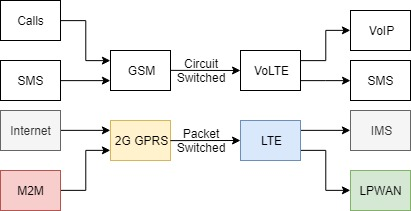
\includegraphics[width=0.5\textwidth,height=\textheight]{C:/GIT/masters/thesis/images/ims voip.jpg}
\caption{A simplified representation of the transition from 2G to LTE
with regard to technologies that keep people and `things' in
contact.\label{fig:2G_LTE_transition}}
\end{figure}

In South Africa, there is a push by cellular service providers to adopt
a cellular LPWAN to fill the void left behind by 2G/GPRS now and in the
future. NB-IoT is being investigated by MTN South Africa, and since they
are also funding this research, have also provided network coverage for
testing to Stellenbosch University. Ideally, the technology can be
rolled out to existing base stations as a software upgrade for national
coverage, but it is limited by factors such as use case demand,
expensive licensing and general uncertainty about the technology.

2G/GPRS has served as the gateway for smart devices and sensors in the
M2M sphere for many years, but due to its high-powered nature it is not
sustainable for applications which require battery longevity of up to 10
years or more. In lieu of its absence, although the spectrum it held can
be re-farmed for cellular LPWANs, it also opens up opportunities for
market entrants of unlicensed frequencies such as LoRaWAN and SigFox.
Each LPWAN technology has its own unique flaws and benefits and there is
yet to be a clear winner when it comes to connecting `things' to the
internet.

When considering rolling out more coverage, since NB-IoT is based off
LTE it makes integration and upgrading of existing infrastructure more
seamless than an entirely separate technology. Although it still retains
the drawbacks and complexities of legacy LTE such as the vast array of
sub-protocols, this still includes the low power, low bandwidth benefits
and others which match the requirements for smart devices and IoT. It
should be mentioned that much of the RF spectrum which can be used for
digital communications is still used by analogue television broadcast by
SABC. ICASA, who controls the spectrum, can solve this issue but over
the years they have been a strong limiting factor as well since they are
slow (if at all) to release new spectrum to MNOs. To increase demand for
application developers in IoT, because they will be interested in a
hands-on approach with the technology they will use, more network
coverage is necessary to scale up production such that volumes of 1000
devices or more can be connected.\footnote{\textbf{history} - from GSM
  in 90s to 5G NB-IoT. \textbf{SA and coverage} - how it ``fits'' in
  South Africa and LPWAN sphere. \textbf{IoT} - how relevent.
  \textbf{coverage} - ICASA. 3GPP - why they designed it. future.
  Uncertainty about NB-IoT. standing. uptake. optimal use}

\hypertarget{coverage}{%
\subsection{Network Coverage}\label{coverage}}

Although NB-IoT joined LPWANs circa 2016-2017, world-wide coverage is
still growing. This can be seen in Fig. \ref{fig:worldwide_coverage}.
\href{https://blog.nordicsemi.com/getconnected/att-launches-nb-iot-network-in-usa}{AT\&T
announced} nation-wide coverage of NB-IoT in the USA, alongside its
existing LTE Cat-M coverage. Deutsche Telekom and Vodafone cover Europe
and China enables millions more IoT devices
{[}\protect\hyperlink{ref-china2019}{3}{]}.

\begin{figure}
\centering
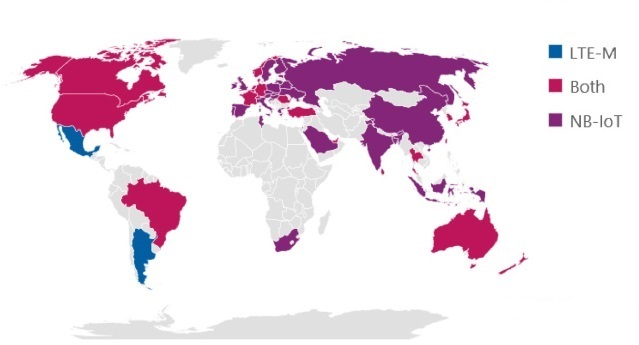
\includegraphics[width=0.9\textwidth,height=\textheight]{../images/countries-deployed-nb-iot-lte-m-networks.jpg}
\caption{Countries with deployed/launched NB-IoT and LTE-M networks
\textcopyright{GSA, 2019} \label{fig:worldwide_coverage}}
\end{figure}

In South Africa, NB-IoT has most of its coverage in the Gauteng province
as well as a few sites in other towns and cities. Although Gauteng only
covers 1.49\% of the land mass in South Africa, it holds
\textasciitilde{}22\% of its \textasciitilde{}57 million people so
understandably it is great as a live trial run before pushing for
national coverage.

\begin{figure}
\centering
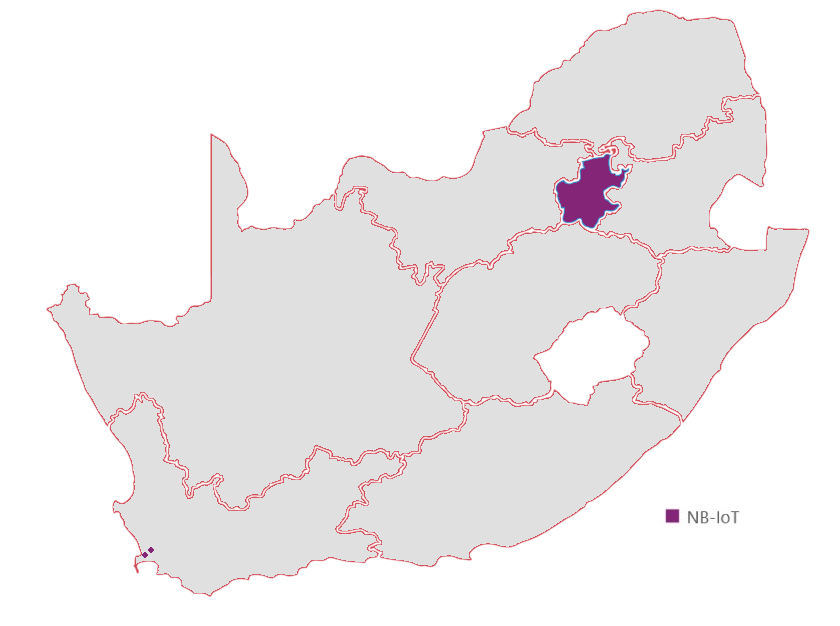
\includegraphics[width=0.5\textwidth,height=\textheight]{../images/GautengvsSouthAfrica.png}
\caption{NB-IoT coverage in South Africa}
\end{figure}

\hypertarget{connectivity}{%
\subsubsection{Connectivity in South Africa}\label{connectivity}}

\begin{tablenos:no-prefix-table-caption}

\begin{longtable}[]{@{}lll@{}}
\caption{NB-IoT connectivity in South Africa with regard to MNO, LTE
vendor and location.}\tabularnewline
\toprule
MNO & LTE Vendor & Location\tabularnewline
\midrule
\endfirsthead
\toprule
MNO & LTE Vendor & Location\tabularnewline
\midrule
\endhead
MTN & ZTE & Stellenbosch\tabularnewline
Vodacom & Nokia & Vodacom Head Office, Cape Town\tabularnewline
MTN & Ericsson & MTN Phase 3: Test Plant\tabularnewline
Vodacom & Huawei & Gauteng Province\tabularnewline
\bottomrule
\end{longtable}

\end{tablenos:no-prefix-table-caption}

To connect via NB-IoT on the Vodacom network, sim cards must be
purchased with a M2M contract over 24 months at 5.00 ZAR/month. At the
time of registering in this study, data bundles range from 5 Mb for 7.50
ZAR to 30 Mb for 29.00 ZAR.

MTN NB-IoT sim cards can currently be obtained only for testing
purposes, and it would be best to speak directly to MTN.

\begin{figure}
\centering
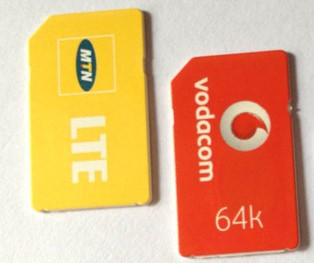
\includegraphics[width=0.3\textwidth,height=\textheight]{../images/LTE-Sims-640-1572213347177.jpg}
\caption{Vodacom and MTN NB-IoT SIM cards}
\end{figure}

\href{../images/MTN-Sim-card.jpg}{}

\hypertarget{iot}{%
\subsection{Internet of Things}\label{iot}}

The internet of things has surged in popularity over recent years as an
interconnected system of devices that transfer data over a network
without requiring human interaction.

Looking at Gartner's analysis of technology expectations with regards to
NB-IoT and related technologies, in 2014 Gartner estimated that Internet
of Things (IoT) had reached the height of inflated expectations, and the
hype it generated lives on in a rich ecosystem of emerging technologies.
As of July 2018, NB-IoT and IoT has falling interest (and hype) in Fig.
\ref{fig:gartner_ictAfrica}, yet it will reach productivity in 2-10
years time. Since new coverage has not been rolled out for almost two
years to date, we believe there is a strong chance for renewed NB-IoT
interest in Africa.

\href{../images/hype-cycle-2014-100371840-large.idge.jpeg}{}

\begin{figure}
\centering
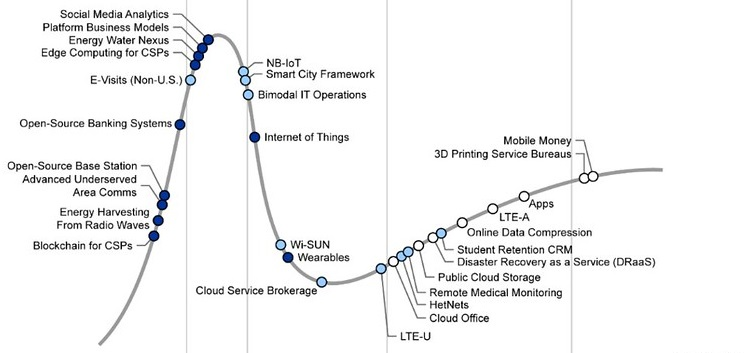
\includegraphics[width=0.9\textwidth,height=\textheight]{../images/42881085945_739bbdc8e9_c.jpg}
\caption{\href{http://www.gartner.com/newsroom/id/3884512}{Gartner's
2018 Hype Cycle for ICT in Africa. NB-IoT is high on the list of
expectations. \label{fig:gartner_ictAfrica}}}
\end{figure}

As of August 2019, Gartner has high expectations for 5G and other
emerging technologies which can make use of what
\href{https://blogs.sas.com/content/hiddeninsights/2016/07/06/long-live-the-iot-hype/}{IoT
has to offer}. This can be seen in Fig. \ref{fig:gartner_emergingTech}.

\begin{figure}
\centering
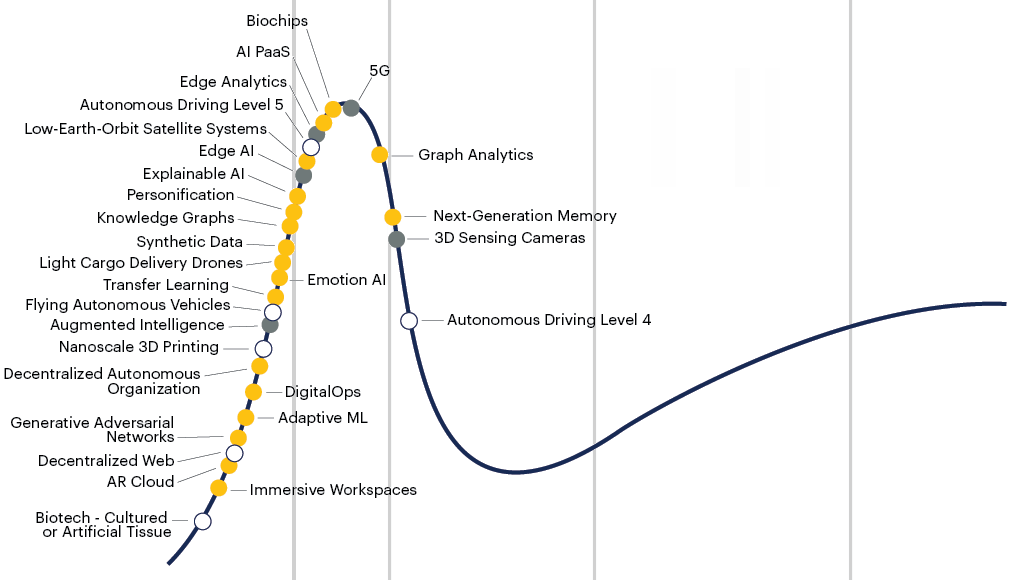
\includegraphics[width=0.9\textwidth,height=\textheight]{../images/CTMKT_741609_CTMKT_for_Emerging_Tech_Hype_Cycle_LargerText-1.png}
\caption{Gartner's Hype Cycle for Emerging Technologies, 2019. IoT is
inextricably linked to at least a third of emerging technologies and
also has uses in NB-IoT. \label{fig:gartner_emergingTech}}
\end{figure}

On the other hand, this does not slow the growth in number of devices
connected as in Fig. \ref{fig:iot_growth}. IoT merely manifests itself
in other uses and forms such as we have already seen in Fig.
\ref{fig:gartner_emergingTech}. NB-IoT can be integral to aid this
growth.

\begin{figure}
\centering
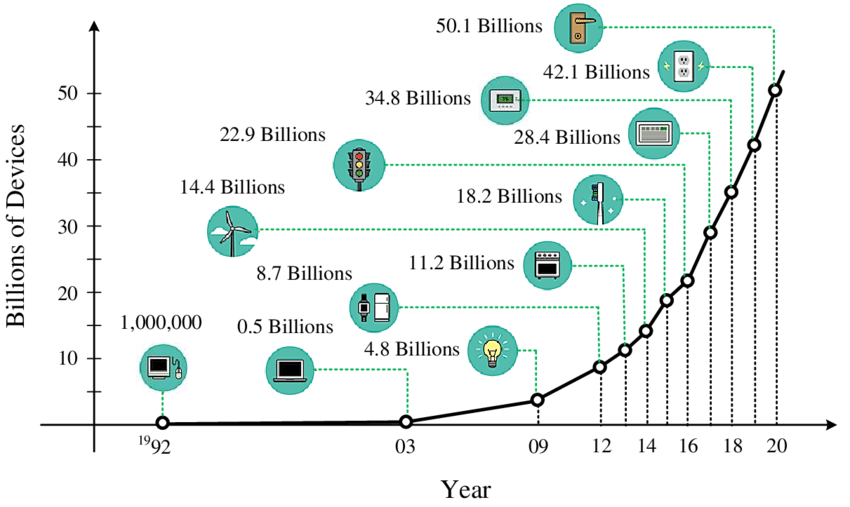
\includegraphics[width=0.8\textwidth,height=\textheight]{../images/Expected-number-of-connected-devices-to-the-Internet-This-chart-is-obtained-from-recent.png}
\caption{Exponential growth of IoT is estimated
{[}\protect\hyperlink{ref-Ali2015}{4}{]}. \label{fig:iot_growth}}
\end{figure}

Matching emerging applications with existing technologies has become one
of the main challenges for IoT initiatives, especially when a new
technology appears in the landscape and the map must be redrawn. Massive
IoT is the deployment of an immense number of low-powered devices with
infrequent reporting and both NB-IoT and LTE Cat-M fulfill the
requirements of 5G massive MTC/IoT.

\hypertarget{lpwans}{%
\subsection{Low-Powered Wide-Area Networks}\label{lpwans}}

There are many wireless technologies out there, with some standardized,
including but not limited to SigFox, LoRaWAN, Dash7, Bluetooth, 6LowPan,
RPMA, Weightless, and IETF 6TiSCH. A brief comparison is drawn on NB-IoT
against prominent unlicensed frequency LPWANs in Table
\ref{tbl:lpwan_comparison}, and cellular LPWANs in Table
\ref{tbl:cellular_comparison}.

\begin{longtable}[]{@{}lllll@{}}
\caption{Brief comparison of NB-IoT against wireless LPWANs
\label{tbl:lpwan_comparison}}\tabularnewline
\toprule
& NB-IoT & LoRaWAN & SigFox & Dash7\tabularnewline
\midrule
\endfirsthead
\toprule
& NB-IoT & LoRaWAN & SigFox & Dash7\tabularnewline
\midrule
\endhead
Frequency & 450-2200 MHz & 433, 868, 915 MHz & 868 MHz & 433, 868, 915
MHz\tabularnewline
Bandwidth & 200 kHz & 125-500 kHz & 200 kHz & 25, 200 kHz\tabularnewline
Throughput & 250 kbps & 27 kbps & 0.1 kbps & 167 kbps\tabularnewline
Duty cycle limitation & 0\% & 90-99\% & 99\% & LBT \textasciitilde{}
0-99\%\tabularnewline
Messages per day (12 B) & 14 million & 10-243 & 140 &
86400+\tabularnewline
Bytes per message & 512 & 255 & 12 & 256\tabularnewline
Uplink Latency & 0.1 - 10 s & \textless{} 3 s & \textasciitilde{} 6 s &
\textless{} 0.015 s\tabularnewline
Battery Lifetime & 10 years & 10 years & 16 years &\tabularnewline
MCL & 164 dBm & 157 dBm & 160 dBm &\tabularnewline
Scalability & & & \textgreater{} 50k &\tabularnewline
Outage & 1\% & \textgreater{} 2\% & 1\% &\tabularnewline
Average Power & & & &\tabularnewline
Range & & 5km (85\% PDR) & 3-10 km &\tabularnewline
\bottomrule
\end{longtable}

\begin{longtable}[]{@{}lllll@{}}
\caption{Brief comparison of NB-IoT against cellular technologies
\label{tbl:cellular_comparison}}\tabularnewline
\toprule
& NB-IoT & 2G/GSM/GPRS & EC-GSM-IoT\footnote{eGPRS/EDGE-based EC-GSM-IoT
  is not available anywhere in the world yet.} & LTE
Cat-M\tabularnewline
\midrule
\endfirsthead
\toprule
& NB-IoT & 2G/GSM/GPRS & EC-GSM-IoT{} & LTE Cat-M\tabularnewline
\midrule
\endhead
Frequencies & 450-2200 MHz & 850-1900 MHz & 850 - 1900 MHz & 450-2600
MHz\tabularnewline
Bandwidth & 180 kHz & 200 kHz & 200 kHz & 1.4MHz\tabularnewline
Throughput & 250 kbps & 56--114 kbps & 70-240 kpbs & 375
kbps\tabularnewline
Packet size & 512 & \textasciitilde{} 1400 & - & \textasciitilde{}
1024\tabularnewline
Uplink Latency & 0.1 - 10 s & 0.3 - 1 s & 0.7 - 2 s & 0.1 - 10
s\tabularnewline
Battery Lifetime & 10 years & 3 months & 10 years & 10
years\tabularnewline
MCL & 164 dBm & 148 dBm & 154 - 164 dBm & 164 dBm\tabularnewline
Scalability & 55,000 & 52,000 & 50,000 & 55,000\tabularnewline
Range (urban) & 2.5 - 5 km & 1 - 2 km & - & 2.5 - 5 km\tabularnewline
\bottomrule
\end{longtable}

To meet application specific requirements, the uniqueness of each
technology gives each its advantages and disadvantages. Matching custom
applications with a wireless technology is non-trivial as there is no
silver bullet that matches all use-cases. In terms of a few metric
capabilities, a best-and-worst case matrix is shown in Table
\ref{tbl:lpwan_strengths}. NB-IoT is shown to be closest to being an
all-round winner, with battery life the exception. This is another
reason why battery life is investigated in this study.

\begin{longtable}[]{@{}lllll@{}}
\caption{LPWAN strengths with \checkmark, \(\times\) denoting best and
worst case respectively. \label{tbl:lpwan_strengths}}\tabularnewline
\toprule
Technology & MCL & Scalability & Battery life &
Throughput\tabularnewline
\midrule
\endfirsthead
\toprule
Technology & MCL & Scalability & Battery life &
Throughput\tabularnewline
\midrule
\endhead
NB-IoT & \checkmark & \checkmark & & \checkmark\tabularnewline
GPRS & \(\times\) & \checkmark & \(\times\) & \checkmark\tabularnewline
LoRaWAN SF7 & & & \checkmark &\tabularnewline
LoRaWAN SF12 & \checkmark & \(\times\) & & \(\times\)\tabularnewline
SigFox & \checkmark & \checkmark & &\tabularnewline
\bottomrule
\end{longtable}

\begin{itemize}
\item
  Competition in the LPWAN space and regional momentum will ensure that
  the various technologies will continue to develop and improve to
  support more features and expand the network coverage.
\item
\item
  Poor for asset tracking and utility metering.
\item
  Average for smart bicyles, parking, garbage bins, agriculture and
  intelligent buildings.
\item
  Good for pet tracking, POS, healthcare.
\item
  NB-IoT outperforms SigFox and LoRaWAN in UL/DL throughput,
  scalability, MCL range and FoTA updates. It is superseded by LoRaWAN
  in battery life for SF7.
\item
  If NB-IoT worked with the mobile network operators to reduce its
  RRC-idle phase, it could develop a minimal power consumption to
  compare with that of LoRaWAN and Sigfox.
\end{itemize}

Although there are many ways to connect IoT to the internet, NB-IoT is
an LPWAN which is the focus of this study.

\hypertarget{metrics_intro}{%
\subsection{Metrics}\label{metrics_intro}}

\begin{itemize}
\tightlist
\item
  \textbf{MCL}: For IoT devices used in extended coverage situations,
  such as deep-indoor devices or remote locations, we recommend either
  Sigfox or NB-IoT, as they offer a maximum MCL of more than 158 dB. IoT
  devices for general use would benefit from the large-scale deployment
  of the GPRS network, which provides excellent coverage because of its
  legacy infrastructure. It is clear that the extra overhead available
  in Sigfox, LoRaWAN, and NB-IoT allows for better indoor coverage than
  GPRS, which means that the LPWAN devices can be used in less than
  optimal operating conditions. Measured MCL correlates with theoretical
  values.
\item
  \textbf{Power consumption}: In applications where device battery life
  is a crucial factor we recommend, either LoRaWAN or Sigfox, because
  they are completely asynchronous. We found that the battery life of
  LoRaWAN SF 7 was five times that of LoRaWAN SF 12 and nearly 25 times
  that of Sigfox. This is mainly due to the extremely long time-on-air
  of LoRaWAN SF 12 and Sigfox. If NB- IoT worked with the mobile network
  operators to reduce its RRC- idle phase, it could develop a minimal
  power consumption to compare with that of LoRaWAN and Sigfox.

  \begin{itemize}
  \tightlist
  \item
    It is clear that LoRaWAN SF7 is the most power-efficient, due to the
    short transmission burst. NB-IoT displays the worst
    power-consumption, due to the extended RRC-idle state. This can be
    reduced using Release Assistance as in Section \ref{release_a}.
  \end{itemize}
\item
  \textbf{Throughput}: As throughput differs greatly between the four
  technologies, comparisons should rather be made in either the licensed
  (NB-IoT and GPRS) or unlicensed (Sigfox and LoRaWAN) spectrum
  categories. Applications that require huge amounts of data to be
  transmitted, such as real-time vehicle fleet monitoring, we recommend
  GPRS and NB-IoT as they are not duty cycle limited. The choice of GPRS
  or NB-IoT will be based on the battery life requirements of the IoT
  device, with NB-IoT having the advantage. In the case of extremely
  low-throughput applications, such as water meters, power meters, and
  weather stations, we recommend Sigfox, as it offers a scalable
  solution with no base station costs involved. Although it limits the
  12 byte throughput per 24 h to 140 messages, this is more than the 20
  messages offered by LoRaWAN SF12 (TTN).

  \begin{itemize}
  \tightlist
  \item
    As NB-IoT operates in the licensed spectrum, there are no throughput
    restrictions, other than the data-rate restriction. We measured the
    uplink and downlink data rates in different signal quality
    environments (distances from the gateway) by querying the modem. The
    measured downlink rate varied from 2250 to 14,193 bps. We could find
    no clear correlation between the downlink data rate and the signal
    quality environment.
  \end{itemize}
\item
  \textbf{Scalability}:

  \begin{itemize}
  \tightlist
  \item
    Lower (sub-500 devices per gateway) scalability of LoRaWAN per base
    station compared to NB-IoT and GPRS. This low scalability is due to
    the limited number of channels and the lack of any scheduling
    between devices. To compensate for the low scalability, an increase
    in spatially diverse base stations would allow packets to be
    received by multiple base stations at varying received power levels.
  \item
    This simulation showed that with 55,000 devices transmitting the
    base station would reach the 270 simultaneously transmitting devices
    that Sigfox claims is possible while still ensuring a 99.9\% PDR.
  \end{itemize}
\item
  \textbf{Down link latency}: In applications where downlink latency is
  a critical component, only GPRS will suffice, as it is the only
  technology in this study that requires constant paging between the
  base station and the end device.
\item
  \textbf{Down link throughput}: Any applications requiring
  bi-directional communication of more than 120 bytes per 24 h, should
  use NB- IoT or GPRS, as Sigfox and LoRaWAN are limited by the duty-
  cycle limitations of the base station.
\item
  \textbf{FoTa}: GPRS and NB-IoT are able to offer FOTA upgrades to IoT
  devices, as Sigfox ha s limited bandwidth. This feature is supported
  by LoRaWAN, through the fragmentation of large payloads {[}22{]}.
\end{itemize}

\hypertarget{usecases_intro}{%
\subsection{Use Cases}\label{usecases_intro}}

\begin{itemize}
\item
  Public Safety
\item
  Agriculture
\item
  Smart Metering
\item
  Actuator Control
\item
  Real-time Monitoring
\item
  Asset Tracking
\item
  Logistics
\item
  Health Care
\item
  Industrial Production
\item
  Energy, Utilities
\item
  Retail
\end{itemize}

IoT has use case requirements in UL/DL throughput, battery longevity and
scalability.

The most popular use case in IoT is smart metering.

\hypertarget{smartmetering}{%
\subsection{Smart Metering}\label{smartmetering}}

One of the simplest use cases in IoT is smart metering. Periodically
sending uplink data at regular intervals from a static location has the
advantage of remote monitoring and reducing the need for physical
readings. It also opened up new features for users (such as dynamic
pricing and usage pattern analysis) and operators (such as load
balancing a large number of clients). The clear value proposition and
success is partially due to the belief that IoT should be low powered
and low data transmissions which still exists today.

\textbf{Smart metering can be considered as defeating the purpose of
NB-IoT when considering its downlink capabilities.}

Smart metering can be considered the traditional IoT model.

\hypertarget{push-pull-model}{%
\subsection{Push-Pull Model}\label{push-pull-model}}

Traditionally, IoT devices push data to the internet at regular
intervals. This push model can be considered quite energy inefficient,
especially when the data is only occasionally actionable. For example,
in asset tracking or remote monitoring.

A pull model is ideal for dynamic rule engines, pulling data only when
necessary and ultimately edge computing, where building an application
around this idea can greatly enhance battery life.

\hypertarget{edge-computing}{%
\subsection{Edge Computing}\label{edge-computing}}

Edge computing is the practice of offloading cloud processes to the
endpoint. It saves on data overhead, especially when there are data
charges involved and battery longevity is desired.

Since NB-IoT is optimized for downlink communications, it can be the
ideal candidate.

\hypertarget{nbiot}{%
\subsection{NB-IoT}\label{nbiot}}

Formed by the 3GPP from LTE, NB-IoT was developed within that framework
and its capabilities are particularly well suited to smart metering.

\begin{figure}
\centering
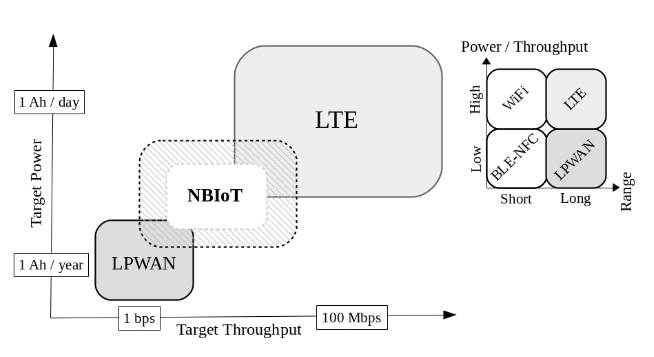
\includegraphics{../images/1559246290186.png}
\caption{IoT Market representation
{[}\protect\hyperlink{ref-Martinez2019}{2}{]}}
\end{figure}

Taking it one step further, the 3GPP defined two device categories,
namely Cat NB1 and NB2, with the latter adding support for:

\begin{itemize}
\tightlist
\item
  Support of Positioning of Device using OTDOA

  \begin{itemize}
  \tightlist
  \item
    seamless cell re-selection
  \end{itemize}
\item
  Push to talk voice messaging
\item
  New Device Power Class (14 dBm)
\item
  Multicast transmission
\end{itemize}

OTDOA positioning,

Compared to LTE

\begin{itemize}
\item
  devices are stationary
\item
  intermittent burst transmissions
\item
  low data bandwidth
\item
  delay-tolerant applications
\item
  support for huge number of devices
\item
  deals with poor coverage (indoor penetration)
\item
  battery lifetime of a few years
\item
  eDRX and PSM
\item
  Debugging

  \begin{itemize}
  \tightlist
  \item
    QXDM, UEMonitor etc
  \item
    {[}\protect\hyperlink{ref-ubloxAppNote2018}{5}{]}
  \end{itemize}
\item
  NB-IoT devices are seen as stationary, only small chunks of data are
  intermittently transmitted and applications are envisaged as
  delay-tolerant.
\item
  NB-IoT technology is designed such that it can be used in areas beyond
  the radio coverage of current cellular standards and in devices which
  must run from battery power for many years. The devices will generally
  send small amounts of data infrequently; a typical usage scenario
  might be 100 to 200 bytes sent twice per day for battery powered
  devices. For mains powered devices the limit is not based on battery
  size, but cost and network bandwidth/resources.
\item
  The system operation is analogous to SMS in that it is a
  datagram-oriented, stored-and-forward system, rather than a GPRS-like
  IP pipe. This is because NB-IoT devices spend most of their time
  asleep, making possible the required long battery life. The system
  implements extended DRX cycles for paging, but as this window will be
  limited to save battery life, the delivery of downlink messages occurs
  mainly when the system detects that uplink messages have been received
  from a device (indicating that it is awake). Here a store-and-forward
  system, an ``IoT Platform'', is useful.
\end{itemize}

Although most users interact only with the UE device which runs its own
proprietary firmware stack, NB-IoT also has a complex backend
architecture.

\hypertarget{lte-architecture}{%
\subsection{LTE Architecture}\label{lte-architecture}}

\begin{figure}
\centering
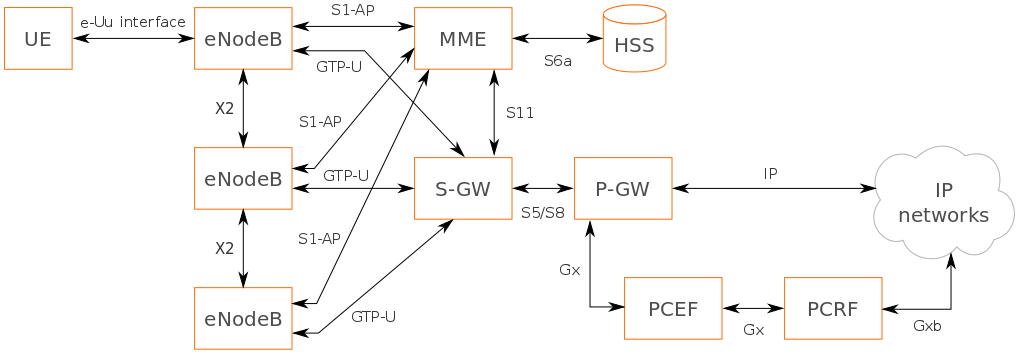
\includegraphics{../images/LTE_classic_architecture.png}
\caption{LTE\_classic\_architecture}
\end{figure}

The complexities of LTE architecture further increases the chance of
performance degradation with respect to 3GPP specifications due to the
vast array of setup parameters. It would be beneficial to analyze the
performance of multiple UE devices against various MNO vendors. It is
important to note that MNOs may use various vendors in their
architecture, and thus this study is mainly focused on the eNodeB vendor
which is also UE device facing and has the greatest chance of
performance degradation due network quality, RF interference and so
forth.

\begin{itemize}
\tightlist
\item
  Both UDP socket commands and datagram commands use the IP data
  transport through the SGi.
\end{itemize}

\hypertarget{performance-evaluation}{%
\subsection{Performance Evaluation}\label{performance-evaluation}}

It would be useful for the application developer to know the boundaries
resulting from this approach. Drawbacks and optimizations targeting IoT
can be discussed. The application developer is a potential adopter of
the technology and focuses on parameters that fall within end-user
control.

Cellular operators would also benefit by knowing where they can improve
upon their configurations and equipment.

To this end it would be beneficial to:

\begin{itemize}
\tightlist
\item
  Analyze critical metrics at the core of NB-IoT, such as energy
  consumption, coverage, cost and latency.
\item
  Create a testing framework to characterize NB-IoT devices in actual
  operation and using various networks.
\item
  Set optimal operating boundaries based on the obtained results. This
  should also re-evaluate suitability in certain use cases.
\end{itemize}

There are over 50 MNOs in the world that are using NB-IoT, yet most draw
from a subset of the
\href{https://www.rcrwireless.com/20160531/network-infrastructure/top-5-wireless-infrastructure-makers-tag4-tag99}{top
5 LTE vendors}:

\begin{enumerate}
\def\labelenumi{\arabic{enumi}.}
\tightlist
\item
  Huawei
\item
  Ericsson
\item
  Nokia
\item
  ZTE
\item
  Samsung
\end{enumerate}

\hypertarget{mno-vendors}{%
\subsection{MNO Vendors}\label{mno-vendors}}

In South Africa, there are two mobile network operators trialing NB-IoT
and combined they use four of the top LTE vendors. Samsung has started
using NB-IoT only as recently as May 2019,
\href{https://enterpriseiotinsights.com/20190506/nb-iot/samsung-kt-launch-nbiot-service-through-ps-lte-network-korea}{announcing
a partnership with KT to create a Public Safety (PS-LTE) network}.
They're also implementing device-to-device (D2D) communications to
increase connectivity in unfavourable conditions.

\begin{longtable}[]{@{}ll@{}}
\caption{MNOs and their BTS Vendors \label{tbl:mno_bts}}\tabularnewline
\toprule
BTS Vendors & Cellular operator (MNO)\tabularnewline
\midrule
\endfirsthead
\toprule
BTS Vendors & Cellular operator (MNO)\tabularnewline
\midrule
\endhead
Nokia & Vodacom\tabularnewline
ZTE & MTN\tabularnewline
Huawei & Vodacom\tabularnewline
Ericsson & MTN\tabularnewline
\bottomrule
\end{longtable}

Theoretically, one can assume that these manufacturers meet 3GPP's
specifications and that they have set up an optimal environment.

With a testing framework, one can evaluate these capabilities in a
transparent manner for both developers and cellular operators alike and
work towards improving the quality thereof.

Cellular operators are in control of some things, and users of others.

\begin{longtable}[]{@{}lll@{}}
\caption{Cellular control \label{tbl:cellular_control}}\tabularnewline
\toprule
& Cellular operators & Users\tabularnewline
\midrule
\endfirsthead
\toprule
& Cellular operators & Users\tabularnewline
\midrule
\endhead
NB-IoT Base stations (BTS) & \textbf{X} &\tabularnewline
NB-IoT User Equipment (UE) & & \textbf{X}\tabularnewline
LoRaWAN Gateways & & \textbf{X}\tabularnewline
LoRaWAN Devices & & \textbf{X}\tabularnewline
NB-IoT licensed spectrum & & billed\tabularnewline
LoRaWAN unlicensed spectrum & & duty-cycled\tabularnewline
& &\tabularnewline
& &\tabularnewline
\bottomrule
\end{longtable}

MNO/BTS Vendors are open to all UE manufacturers.

Other Vendors include: Broadcom Corporation, Cisco Systems, Gemalto NV,
Intel Corporation, KDDI Corporation, LG Electronics, MediaTek, Oberthur
Technologies, Ooredoo, Orange, Samsung Electronics, Saudi Telecom
Company, Sierra Wireless, Telit Communications and VimpelCom.

\hypertarget{ue-manufacturers}{%
\subsection{UE Manufacturers}\label{ue-manufacturers}}

UE devices specifically used:

\begin{itemize}
\tightlist
\item
  Ublox Sara N200
\item
  Quectel BC95
\end{itemize}

and the following recommended in future:

\begin{itemize}
\tightlist
\item
  Nordic nRF9160
\item
  SimCom SIM7020E
\end{itemize}

\hypertarget{ublox}{%
\subsubsection{Ublox}\label{ublox}}

\hypertarget{quectel}{%
\subsubsection{Quectel}\label{quectel}}

\hypertarget{nordic}{%
\subsubsection{Nordic}\label{nordic}}

\hypertarget{simcom}{%
\subsubsection{SimCom}\label{simcom}}

These UEs all share AT commands as the API to control their
capabilities.

\hypertarget{atcommands}{%
\subsection{AT Commands}\label{atcommands}}

This section outlines the capabilities of the UEs.

\begin{tablenos:no-prefix-table-caption}

\begin{longtable}[]{@{}lll@{}}
\caption{Summary AT Command set for Ublox }\tabularnewline
\toprule
\begin{minipage}[b]{0.20\columnwidth}\raggedright
\strut
\end{minipage} & \begin{minipage}[b]{0.10\columnwidth}\raggedright
Command\strut
\end{minipage} & \begin{minipage}[b]{0.61\columnwidth}\raggedright
Description\strut
\end{minipage}\tabularnewline
\midrule
\endfirsthead
\toprule
\begin{minipage}[b]{0.20\columnwidth}\raggedright
\strut
\end{minipage} & \begin{minipage}[b]{0.10\columnwidth}\raggedright
Command\strut
\end{minipage} & \begin{minipage}[b]{0.61\columnwidth}\raggedright
Description\strut
\end{minipage}\tabularnewline
\midrule
\endhead
\begin{minipage}[t]{0.20\columnwidth}\raggedright
Set configuration\strut
\end{minipage} & \begin{minipage}[t]{0.10\columnwidth}\raggedright
AT+NCONFIG\strut
\end{minipage} & \begin{minipage}[t]{0.61\columnwidth}\raggedright
Change configuration for SI\_AVOID, Scrambling etc.\strut
\end{minipage}\tabularnewline
\begin{minipage}[t]{0.20\columnwidth}\raggedright
Network Registration\strut
\end{minipage} & \begin{minipage}[t]{0.10\columnwidth}\raggedright
AT+COPS\strut
\end{minipage} & \begin{minipage}[t]{0.61\columnwidth}\raggedright
This command initiates search for cell towers to connect to depending on
MNO-related SIM-card and registers/deregisters accordingly.\strut
\end{minipage}\tabularnewline
\begin{minipage}[t]{0.20\columnwidth}\raggedright
Set APN\strut
\end{minipage} & \begin{minipage}[t]{0.10\columnwidth}\raggedright
AT+CGDCONT\strut
\end{minipage} & \begin{minipage}[t]{0.61\columnwidth}\raggedright
Sets the relevant APN for the MNO.\strut
\end{minipage}\tabularnewline
\begin{minipage}[t]{0.20\columnwidth}\raggedright
\strut
\end{minipage} & \begin{minipage}[t]{0.10\columnwidth}\raggedright
\strut
\end{minipage} & \begin{minipage}[t]{0.61\columnwidth}\raggedright
\strut
\end{minipage}\tabularnewline
\bottomrule
\end{longtable}

\end{tablenos:no-prefix-table-caption}

\begin{itemize}
\tightlist
\item
  SARA-N2 series modules implement a FOTA solution based on CoAP. It is
  possible to configure the module's poll timer for when the module
  checks the FOTA CoAP server for new firmware. When the feature is
  enabled and a new package is available, the module will automatically
  download the FOTA update and provide URCs about its progress. The
  module's firmware is not updated automatically when the download has
  completed and so the application must start the upgrade process step.
\item
  The +UTEST AT command allows the user to set the module in
  non-signaling (or test) mode, or returns to the signaling (or normal)
  mode. In test/non-signaling mode, the module switches off the protocol
  stack for performing single tests which could not be performed during
  the signaling mode.
\item
  MO Datagrams sent and received by IoT platform has these commands
  wrapped internally in a Constrained Application Protocol (CoAP)
  message and sent over UDP sockets. Once the module accepted a datagram
  it cannot be removed and will be transmitted to the network as soon as
  radio conditions permit. The only way to clear the module's transmit
  queue is to reboot it. In good radio conditions, the transmission
  might take a few seconds. In bad radio conditions a transmission
  opportunity may not occur for minutes, days or weeks but the datagram
  will be transmitted once radio conditions are good enough. When a MO
  message is queued, the module will try to send the message to the base
  station. It will only send the next message once the previous message
  has been sent. If there is a radio link failure (RLF), the device will
  re-scan the channel ranges and try to reconnect to a base station.
  There may be a back off time where the device goes into deep-sleep
  mode before trying again.
\item
  An unsolicited result code (URC) is a string message (provided by the
  DCE) that is not a response to a previous AT command. It can be
  output, when enabled, at any time to inform the DTE of a specific
  event or status change.
\end{itemize}

When it comes to base stations, the user does not have control over the
inactivity timer. Release assistance can request the eNB/network to
disconnect the modem from Radio Resource Control (RRC) connected mode.

\hypertarget{thesis-struct}{%
\subsection{Thesis structure}\label{thesis-struct}}

NB-IoT is introduced to the reader in Chapter \ref{intro}. A literature
study reviews the current empirical research in Chapter \ref{litstudy}.
Design and methodology shows the steps taken to capture different
metrics and process the resulting dataset in Chapter \ref{design}.
Results are analyzed in Chapter \ref{results} and discussed with
recommendations in Chapter \ref{#discussion}. Lastly, a conclusion is
made in Chapter \ref{conclusion}.

\newpage

\hypertarget{notes}{%
\section{Notes}\label{notes}}

\begin{itemize}
\tightlist
\item
  rename MNO vendors to LTE vendors?
\end{itemize}

\newpage

\hypertarget{references}{%
\section*{References}\label{references}}
\addcontentsline{toc}{section}{References}

\hypertarget{refs}{}
\leavevmode\hypertarget{ref-Durand2019}{}%
{[}1{]} T. Durand, L. Visagie, and M. Booysen, ``Evaluation of
next-generation low-power communication technology in
IoT-applications,'' \emph{IET Communications}, pp. 1--8, 2019.

\leavevmode\hypertarget{ref-Martinez2019}{}%
{[}2{]} B. Martinez, S. Member, F. Adelantado, A. Bartoli, and X.
Vilajosana, ``Exploring the Performance Boundaries of NB-IoT.''

\leavevmode\hypertarget{ref-china2019}{}%
{[}3{]} U. Enable, M. More, and I. Devices, ``NB-IoT Commercialisation
Case Study How China Mobile , China Telecom and China.''

\leavevmode\hypertarget{ref-Ali2015}{}%
{[}4{]} A. Ali, W. Hamouda, and M. Uysal, ``Next generation M2M cellular
networks: Challenges and practical considerations,'' \emph{IEEE
Communications Magazine}, vol. 53, no. 9, pp. 18--24, 2015.

\leavevmode\hypertarget{ref-ubloxAppNote2018}{}%
{[}5{]} A. Note, ``NB-IoT Application Development Guide.''

\end{document}
